\documentclass{beamer}
\usetheme[pageofpages=of,% String used between the current page and the
                         % total page count.
          bullet=circle,% Use circles instead of squares for bullets.
          titleline=true,% Show a line below the frame title.
          alternativetitlepage=true,% Use the fancy title page.
       %   titlepagelogo=logo-polito,% Logo for the first page.
       %   watermark=watermark-polito,% Watermark used in every page.
       %   watermarkheight=100px,% Height of the watermark.
       %   watermarkheightmult=4,% The watermark image is 4 times bigger
                                % than watermarkheight.
          ]{Torino}

\setbeamertemplate{footline}{
  \begin{beamercolorbox}[wd=\paperwidth,ht=1ex,dp=1ex]{footline}
    \vspace{5pt} \hspace{1em} \insertframenumber/\inserttotalframenumber
  \end{beamercolorbox}
}

\author{Brendon J. Brewer}
\title{STATS 331 -- Introduction to Bayesian Statistics}
\institute{The University of Auckland}
\date{}


\linespread{1.3}
\usepackage{minted}
\usepackage[utf8]{inputenc}
\usepackage{dsfont}
\newcommand{\given}{\,|\,}

\begin{document}

\frame{\titlepage}

\begin{frame}
\begin{center}
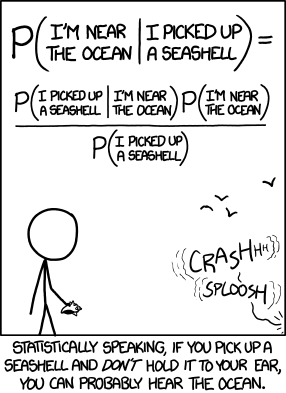
\includegraphics[width=0.4\textwidth]{images/seashell.png}
\end{center}

Randall Monroe, xkcd.com

\end{frame}


\begin{frame}

\begin{center}
\Large
Bigger Bayes' Boxes and \\
Introduction to Parameter Estimation
\end{center}

\end{frame}



\begin{frame}
\frametitle{Medical Testing Example}


    \begin{columns} % Create two columns
        \column{0.7\textwidth} % Left column (50% width)

        \begin{itemize}
        \item There is a disease $A$ and your prior
                probability of having it is 0.01,
                given that you have the symptoms.

        \item   There is a test which tells you
                whether you have $A$, but with 5\%
                probability the test result is flipped.

        \item The test is also sensitive to the
                more common disease $B$, and you
                have a 0.05 prior probability of
                having that.
        \end{itemize}

        \column{0.3\textwidth} % Right column (50% width)
        
\includegraphics[width=0.6\linewidth]{images/medicine.jpg}
       
         (public domain image)
     \end{columns}

\end{frame}


\begin{frame}
\frametitle{The Data}

\begin{itemize}
\item The test result is the data. $D$ = ``The test comes back positive''.\pause
\item How plausible is it that you have $A$? \pause
\item Difficulty: need list of mutually exclusive hypotheses
        to make a Bayes' Box. How do we get $B$ involved? \pause
\item Solution: Use logical AND. Four possibilities:
        You have $A$ only, $B$ only, both, or neither.
        Assume independence to get the prior
        probabilities of these.
\end{itemize}

\end{frame}




\begin{frame}
\frametitle{Bayes' Box}
Setting up the prior column of the Bayes' Box using independence:
\vspace{1em}

\begin{tabular}{|c|c|c|c|c|}
\hline
Hypothesis & Prior & Likelihood & Prior $\times$ Likelihood & Posterior \\
\hline
$A$ only & 0.01 $\times$ 0.95 & & & \\
$B$ only & 0.99 $\times$ 0.05 & & & \\
Both     & 0.01 $\times$ 0.05 & & & \\
Neither  & 0.99 $\times$ 0.95 & & & \\
\hline
Total & 1 & & & \\
\hline
\end{tabular}


\end{frame}


\begin{frame}
\frametitle{Bayes' Box}
Setting up the likelihood column of the Bayes' Box using the information
about test reliability:
\vspace{1em}

\begin{tabular}{|c|c|c|c|c|}
\hline
Hypothesis & Prior & Likelihood & Prior $\times$ Likelihood & Posterior \\
\hline
$A$ only & 0.01 $\times$ 0.95 & 0.95 & & \\
$B$ only & 0.99 $\times$ 0.05 & 0.95 & & \\
Both     & 0.01 $\times$ 0.05 & 0.95 & & \\
Neither  & 0.99 $\times$ 0.95 & 0.05 & & \\
\hline
Total & 1 & & & \\
\hline
\end{tabular}

\pause
\vspace{0.3em}
Which hypothesis would ``maximum likelihood estimation''
select?


\end{frame}


\begin{frame}[fragile]
\frametitle{The Calculation Process in R}

\begin{minted}{r}
> prior = c(0.01*0.95, 0.99*0.05, 0.01*0.05, 0.99*0.95)
> prior
[1] 0.0095 0.0495 0.0005 0.9405
> lik = c(0.95, 0.95, 0.95, 0.05)
> h = prior*lik
> Z = sum(h)
> Z
[1] 0.10355
> post = h/Z
> post
[1] 0.087155963 0.454128440 0.004587156 0.454128440
\end{minted}

\end{frame}


\begin{frame}
\frametitle{Medical Testing Example: Conclusion}
It is most plausible that you have either $B$ or nothing.

\end{frame}


\begin{frame}
\frametitle{Bayes' Rule for Sets of Hypotheses}
Suppose we have a set of mutually exclusive and exhaustive hypotheses
$H_1, ..., H_n$. This means one and only one of them is true --- this is usually
the way things are initially arranged and the medical testing example was an
exception.\pause

Bayes' rule for the posterior probability of each hypothesis $H_i$:
\begin{align}
P(H_i \given D) &= \frac{P(H_i)P(D \given H_i)}{P(D)}
\end{align}\pause
The marginal likelihood involves a sum over all hypotheses:
\begin{align}
P(D) &= \sum_{i=1}^n P(H_i)P(D \given H_i).
\end{align}

\end{frame}


\begin{frame}
\frametitle{Bayes' Rule $n$ times $\equiv$ Bayes' Box}
Using a Bayes' Box with $n$ rows and applying the procedure there
(once you have assigned priors and likelihoods) is equivalent
to using Bayes' rule $n$ times and the marginal likelihood formula
as given on the previous slide.

\end{frame}

\begin{frame}

\begin{center}
\Large
Parameter Estimation
\end{center}

\end{frame}


\begin{frame}
\frametitle{Parameter Estimation}

\begin{itemize}
\item Parameter estimation is a really important part of statistics.\pause
\item A parameter is {\bf a quantity whose value we would like to
        know.}\footnote{It's a bit more than this, but this will do for now.}\pause
\item We will describe our uncertainty about the value of the parameter
using a {\bf probability distribution}.\pause
\item This gets updated from a {\bf prior distribution}
    to a {\bf posterior distribution}
    as we get more information.
\end{itemize}

\end{frame}

\begin{frame}
\frametitle{Parameter Estimation}
Recall that Bayes' rule can be used on a set of mutually exclusive hypotheses.
These can be statements about the value of the parameter $\theta$.\pause

\begin{itemize}
\item One hypothesis might be ``$\theta = 1$'' \pause
\item Another might be ``$\theta = 2$'' \pause
\item We might get some data like ``$x = 3$''.
\end{itemize}

\end{frame}


\begin{frame}
\frametitle{Bayes' Rule Lots of Times}
\begin{align}
P(\theta = 1 \given x = 3) &= \frac{P(\theta=1)P(x=3 \given \theta=1)}{P(x=3)}\\
P(\theta = 2 \given x = 3) &= \frac{P(\theta=2)P(x=3 \given \theta=2)}{P(x=3)}\\
&...&\\
P(\theta = 9 \given x = 3) &= \frac{P(\theta=9)P(x=3 \given \theta=9)}{P(x=3)}\\
\end{align}

\end{frame}

\begin{frame}
\frametitle{Bayes' Rule Lots of Times}
\begin{align}
\color{red}{P(\theta = 1 \given x = 3)} &= \frac{{\color{blue}P(\theta=1)}P(x=3 \given \theta=1)}{P(x=3)}\\
\color{red}{P(\theta = 2 \given x = 3)} &= \frac{{\color{blue}P(\theta=2)}P(x=3 \given \theta=2)}{P(x=3)}\\
&...&\\
\color{red}{P(\theta = 9 \given x = 3)} &= \frac{{\color{blue}P(\theta=9)}P(x=3 \given \theta=9)}{P(x=3)}\\
\end{align}

{\color{red}Posterior Distribution}
{\color{blue}Prior Distribution}

\end{frame}


\begin{frame}
\frametitle{Bayes' Rule Lots of Times}
\begin{align}
P(\theta = 1 \given x = 3) &= \frac{P(\theta=1){\color{orange}P(x=3 \given \theta=1)}}{\color{green}P(x=3)}\\
P(\theta = 2 \given x = 3) &= \frac{P(\theta=2){\color{orange}P(x=3 \given \theta=2)}}{\color{green}P(x=3)}\\
&...&\\
P(\theta = 9 \given x = 3) &= \frac{P(\theta=9){\color{orange}P(x=3 \given \theta=9)}}{\color{green}P(x=3)}\\
\end{align}

{\color{orange}Likelihood Function}
{\color{green}Marginal Likelihood (common to all $\theta$ values)}

\end{frame}

\begin{frame}
\frametitle{Bayes' Box for Parameter Estimation}
Since a Bayes' Box is equivalent to these repeated uses of Bayes' rule,
we can use them for parameter estimation (when there is only one unknown
parameter).

\end{frame}


\begin{frame}
\frametitle{Example Bayes' Box for Parameter Estimation}
\begin{tabular}{|c|c|c|c|c|}
\hline
Parameter & Prior & Likelihood & Prior $\times$ Likelihood & Posterior \\
$\theta$  & $p(\theta)$ & $p(x \given \theta)$ & $p(\theta)p(x\given\theta)$ & $p(\theta\given x)$ \\
\hline
0.1 & 0.2  &  & & \\
0.2 & 0.2  &  & & \\
0.3 & 0.2 &  & & \\
0.4 & 0.2  &  & & \\
0.5 & 0.2 & & & \\
\hline
Total & 1 & & & 1 \\
\hline
\end{tabular}
\pause
\vspace{1em}

Note the notation for the columns with the lower case $p$
which means ``probability distribution for''.


\end{frame}


\begin{frame}
\frametitle{Bayes' Rule for Parameter Estimation}
Instead of writing down Bayes' rule lots of times, we often write it down
once only, with each term being a whole function of $\theta$ not just
a single probability.\pause
\begin{align}
p(\theta \given x) &= \frac{p(\theta)p(x \given \theta)}{p(x)} \\
p(\theta \given x) &\propto p(\theta)p(x \given \theta) \\
\texttt{posterior} &\propto \texttt{prior} \times \texttt{likelihood}
\end{align}
\pause
(notation: $\theta$=parameter, $x$=data)
We will use this more when we do {\bf analytical methods}. For now, we will
stick to the Bayes' Box.


\end{frame}


\begin{frame}
\frametitle{What Usually Happens}
Usually, the prior distribution $p(\theta)$ is something wide (indicating
a lot of uncertainty). After analysing data we get the posterior distribution
$p(\theta \given x)$ which is usually narrower than the prior.

\begin{center}
\includegraphics[width=0.5\textwidth]{images/updating.pdf}
\end{center}

\end{frame}


\begin{frame}
\frametitle{Estimating a Proportion}

\begin{itemize}
\item We will now solve the famous problem of estimating a
proportion using a Bayes' Box.\pause
\item Suppose there is an election coming up, with two major
parties. 10 people are called to take a poll.\pause
\item Results (data): $\{1, 1, 0, 0, 1, 0, 1, 0, 1, 1\}$\pause
\item What fraction $\theta$ of the entire population supports the party
represented by `1' in the data?
\end{itemize}

\end{frame}

\begin{frame}
\frametitle{Estimating a Proportion --- Uniform Prior}

\centering
{\footnotesize
\begin{tabular}{|c|c|c|c|c|}
\hline
Parameter & Prior & Likelihood & Prior $\times$ Likelihood & Posterior \\
$\theta$  & $p(\theta)$ & $p(x \given \theta)$ & $p(\theta)p(x\given\theta)$ & $p(\theta\given x)$ \\
\hline
0 & 0.0909 & & & \\
0.1 & 0.0909  &  & & \\
0.2 & 0.0909  &  & & \\
0.3 & 0.0909 &  & & \\
0.4 & 0.0909  &  & & \\
0.5 & 0.0909 & & & \\
0.6 & 0.0909 & & & \\
0.7 & 0.0909 & & & \\
0.8 & 0.0909 & & & \\
0.9 & 0.0909 & & & \\
1   & 0.0909 & & & \\
\hline
Total & 1 & & & 1 \\
\hline
\end{tabular}
}

\end{frame}


\begin{frame}[fragile]
\frametitle{Creating the Parameter and Prior Vectors in R}
We will often use R's \mintinline{r}{seq()} and
\mintinline{r}{rep()} functions to do this.\pause

\begin{minted}{r}
theta = seq(0, 1, by=0.1)
prior = rep(1/length(theta), length(theta))
\end{minted}

\end{frame}

\begin{frame}
\frametitle{Likelihood}
We called 10 people and the data was
$\{1, 1, 0, 0, 1, 0, 1, 0, 1, 1\}$. We can reason out the likelihood
--- imagining we know $\theta$, but leaving it as a symbol, so we get
all likelihood values at once.\pause
\begin{align}
P(1 \given \theta) &= \theta \\
P(0 \given \theta) &= 1-\theta \\
P(\{1, 1, 0\} \given \theta) &= \theta\theta(1-\theta) \\
P(\{1, 1, 0, 0, 1, 0, 1, 0, 1, 1\}) &= \theta^6(1-\theta)^4
\end{align}



\end{frame}

\begin{frame}
\frametitle{Likelihood}
In the beginning of this course, finding likelihoods is the hardest
part for many students. Put yourself in the hypothetical situation
of knowing $\theta$ but not knowing the data, and ask yourself
what the probability would be of the data that you got.\\[1em]\pause

Later, this will get easier, when we use
{\bf sampling distributions}
as a stepping stone to getting the likelihood function.

\end{frame}

\begin{frame}[fragile]
\frametitle{Likelihood in R}
We have a formula involving $\theta$, so we can simply use it
in R:

\begin{minted}{r}
lik = theta^6*(1-theta)^4
\end{minted}

\end{frame}

\begin{frame}[fragile]
\frametitle{Solution in R}

\begin{minted}{r}
theta = seq(0, 1, by=0.1)
prior = rep(1/length(theta), length(theta))
lik = theta^6*(1-theta)^4
h = prior*lik
Z = sum(h)
post = h/Z
\end{minted}
\end{frame}


\begin{frame}
\frametitle{Solution --- Plot}

\centering
\includegraphics[width=0.7\textwidth]{images/election.pdf}

\end{frame}


\begin{frame}
\frametitle{A Note on Constant Factors in the Likelihood}

\begin{itemize}
\item The bus problem in the notes is very closely related to
this. It uses the binomial distribution as the sampling distribution, from
which we get the likelihood.\pause
\item This is appropriate if you only know about the 6
successes (out of the 10 trials), rather than the full
sequence of successes and failures.\pause
\item The only difference in the formula for the
likelihood is a constant out the front (not involving $\theta$).\pause
\item The likelihoods and marginal likelihood are affected by this constant,
but because we divide by the marginal likelihood, the posterior is the same
whether the constant is there or not.
\end{itemize}

\end{frame}


\begin{frame}
\frametitle{Outputs Again}

\begin{itemize}
\item Recall that the outputs of Bayesian calculations are the posterior distribution
and the marginal likelihood.\pause
\item These --- especially the posterior distribution --- are the complete
answer to the inference problem.
\end{itemize}

\centering

\includegraphics[width=0.3\textwidth]{images/brosh.jpg}

{\tiny (Image credit: Allie Brosh)}

\end{frame}


\end{document}

